\chapter{\textit{Branch-and-Cut}}
A formulação do TSP proposta por requer uma quantidade exponencial de espaço dada a natureza das restrições de \textit{subtour}. Contudo, como será mostrado nesse capítulo, nem todas as restrições são necessárias para se obter a solução ótima. Em outras palavras, as restrições --- ou cortes --- de \textit{subtour} podem ser geradas algoritmicamente ``sob demanda".

\section{\textit{Lazy constraints}}
Considere a seguinte formulação do TSP, sem as restrições de \textit{subtour}:

\begin{align*}
    \text{min }& \sum_{i \in V}\sum_{j \in V, j > i}c_{ij} x_{ij} &\\
    \text{s.a }& \sum_{j \in V, j < i}x_{ij}  +  \sum_{j \in V, j > i}x_{ij} = 2  &\forall i \in V \\
    & x_{ij} \in \{0, 1\} &\forall i, j \in V
    \label{TSPsemsub}
\end{align*}

Utilizando-a como modelo, um \textit{solver} produziria uma solução de estrutura semelhante às das soluções do algoritmo húngaro utilizado no Capítulo 2 --- que possuem o somatório de pesos de arestas mínimo, mas que não garantem um único \textit{tour}. 

A partir da mesma formulação, uma instância com 6 nós, por exemplo, poderia gerar uma solução \(s = \{\{1,3,5\}, \{2,4,6\}\}\). Os dois \textit{subtours} são indesejados, e após detectados, podem ser removidos adicionando-se as seguintes restrições 
\begin{align}
    x_{13} + x_{35} + x_{51} &\leq 3 - 1 \\  
    x_{24} + x_{46} + x_{62} &\leq 3 - 1 
\end{align}
e resolvendo o problema novamente.

Se, ao resolver o problema novamente, uma solução ótima \(s = \{1, 3, 5, 2, 4 , 6\}\), fosse obtida, saberia-se que ela é a solução ótima do problema original, pois por conter apenas um \textit{tour}, ela atende a todas as restrições de \textit{subtour} implicitamente, mesmo que nem todas elas tenham sido usadas pelo \textit{solver} durante a resolução.

As restrições 1 e 2 são chamadas de \textit{lazy constraints}, pois ainda que sejam \textit{necessárias} na procura de uma solução viável, são adicionadas apenas quando uma solução inteira que não satisfaz as restrições de \textit{subtour} é encontrada.

Dessa forma, uma maneira de implementar um  algoritmo exato que faz uso da noção de restrições sob demanda é utilizar a formulação matemática de sem as restrições de \textit{subtour}. Após isso, sempre que uma solução ótima for obtida, pode-se utilizar um algoritmo simples de detecção de \textit{subtours}\footnote{Tais algoritmos também podem ser chamados de algoritmos de separação, pois são capazes de separar uma solução inteira inviável do poliedro que descreve o problema ao adicionar restrições que a proiba.}, e proibi-los por meio da adição de restrições ao modelo e resolvê-lo novamente, até que uma solução inteira que contenha apenas um \textit{tour} seja obtida.

\section{\textit{Min-Cut}}
Dado um grafo \(G = (V, E)\), se \(V\) é dividido em dois subconjuntos disjuntos \(V_1\) e \(V_2\) tais que \(V_1 \cup V_2 = V\), diz-se que a partição \(\{V_1, V_2\}\) é um corte de \(G\). Suponha agora que \(G\) seja um grafo completo, e que \(K\) seja o conjunto de arestas compartilhadas por \(V_1\) e \(V_2\). Se \(\sum_{e \in K}c_e\) é o mínimo possível, diz-se que a partição \(\{V_1, V_2\}\) é um corte mínimo ou \textit{min-cut} de \(G\).

Dois métodos diferentes de obter o corte mínimo de um grafo serão apresentados nas próximas seções.

\section{Cortes em um poliedro}
Durante a resolução de um ILP como o TSP, \textit{solvers} como o \textit{CPLEX} fazem uso de algoritmos BB. Mais precisamente, relaxações lineares do problema original são tratadas como subproblemas, e escolhe-se as variáveis mais fracionárias para realizar o \textit{branching}, que consiste em adicionar restrições de integralidade a essas variáveis. Dessa forma, o \textit{CPLEX} itera sobre soluções fracionárias até que uma solução inteira seja obtida. 

Como visto anteriormente, se a solução inteira violar as restrições de \textit{subtour}, pode-se utilizar um algoritmo de separação e adicionar as restrições violadas até que uma solução inteira viável --- e consequente ótima, nesse caso --- seja obtida. Acontece que, utilizando-se a  mesma noção, é possível adicionar restrições no problema durante a resolução da relaxação linear (subproblema). 

Na Figura \ref{poliedros}, o maior poliedro representa a relaxação linear do problema original. Adicionando-se mais restrições, é possível ``cortar" o poliedro original, aproximando-o mais da envoltória convexa de \(P\). Por esse motivo, tais restrições adicionais também são chamadas de cortes\footnote{Observe que, embora estejam relacionados nesse contexto, cortes em um poliedro são totalmente diferentes de cortes de um grafo.}.

\begin{figure}[h]
    \centering
    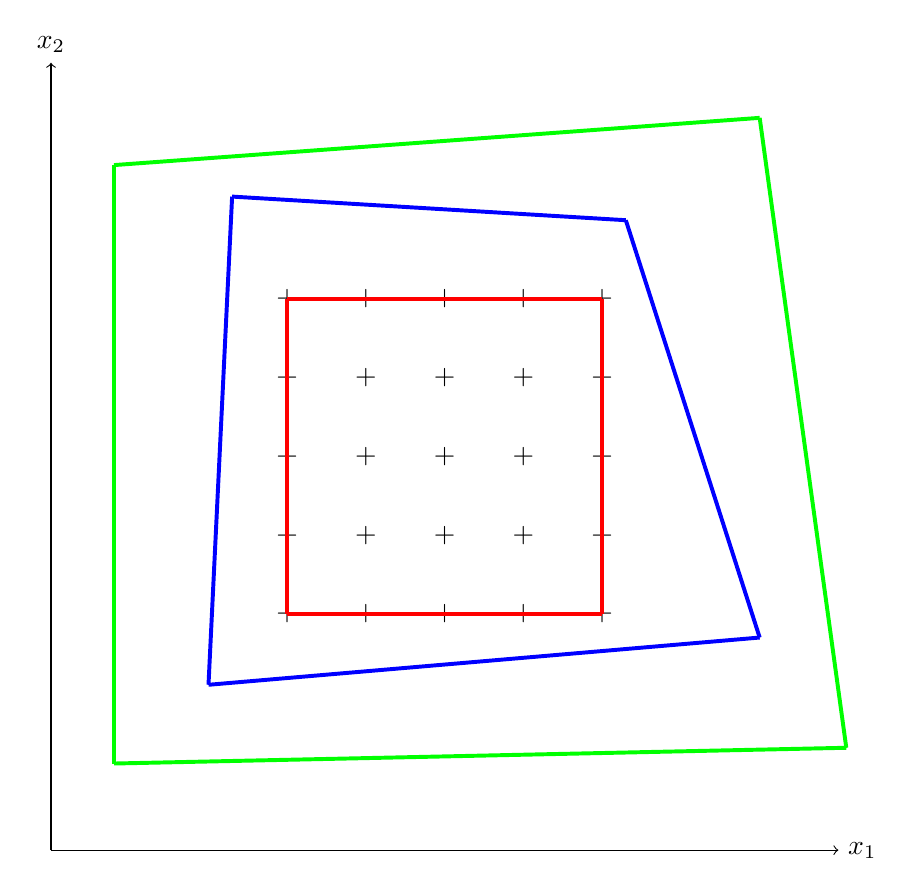
\begin{tikzpicture}
    
    \node (s1) at (3,3) {+};
    \node (s2) at (4,3) {+};
    \node (s3) at (5,3) {+};
    \node (s3) at (6,3) {+};    
    \node (s3) at (7,3) {+};
    \node (s1) at (3,4) {+};
    \node (s2) at (4,4) {+};
    \node (s3) at (5,4) {+};
    \node (s3) at (6,4) {+};    
    \node (s3) at (7,4) {+};   
    \node (s1) at (3,5) {+};
    \node (s2) at (4,5) {+};
    \node (s3) at (5,5) {+};
    \node (s3) at (6,5) {+};    
    \node (s3) at (7,5) {+};   
    \node (s1) at (3,6) {+};
    \node (s2) at (4,6) {+};
    \node (s3) at (5,6) {+};
    \node (s3) at (6,6) {+};    
    \node (s3) at (7,6) {+};   
    \node (s1) at (3,7) {+};
    \node (s2) at (4,7) {+};
    \node (s3) at (5,7) {+};
    \node (s3) at (6,7) {+};    
    \node (s3) at (7,7) {+};   

    \draw[-][line width=0.5mm, red ]  (3,3)--(7,3);
    \draw[-][line width=0.5mm, red ]  (7,7)--(7,3);
    \draw[-][line width=0.5mm, red ]  (3,3)--(3,7);
    \draw[-][line width=0.5mm, red ]  (3,7)--(7,7);

    \draw[-][line width=0.5mm, blue ]  (2,2.1)--(9,2.7);
    \draw[-][line width=0.5mm, blue ]  (2.3,8.3)--(7.3,8);
    \draw[-][line width=0.5mm, blue ]  (2,2.1)--(2.3,8.3);
    \draw[-][line width=0.5mm, blue ]  (7.3,8)--(9,2.7);
    
    \draw[-][line width=0.5mm, green ]  (0.8,1.1)--(10.1,1.3);
    \draw[-][line width=0.5mm, green ] (10.1,1.3)--(9,9.3);
    \draw[-][line width=0.5mm, green ]  (9,9.3)--(0.8, 8.7);
    \draw[-][line width=0.5mm, green ]  (0.8, 8.7)--(0.8,1.1);

    \draw[->] (0,0)--(0,10) node[above] {$x_2$};
    \draw[->] (0,0)--(10,0) node[right] {$x_1$};

    
    \end{tikzpicture} 
    

    \caption{Poliedros.}
    \label{poliedros}
\end{figure}

\section{Cortes no TSP}
Uma solução fracionária para a relaxação linear do TSP sem restrição de \textit{subtours} pode ser interpretada como um grafo completo. No grafo, todas as arestas terão um peso que varia de \(0\) a \(1\), e que obedecem às restrições de grau.
Suponha que, ao resolver a versão relaxada do TSP,  um \textit{solver} chegue a uma solução fracionária cujo corte mínimo é ilustrado na Figura \ref{fig:solucaoFrac}. Nela, o somatório dos pesos das arestas compartilhadas por \(S\) e \(\overline{S}\) é maior que \(2\). Isso significa que a solução, mesmo que fracionária, obedece a todas as restrições de \textit{subtour}, já que o corte mostrado é o menor possível. 

\begin{figure}[h]
    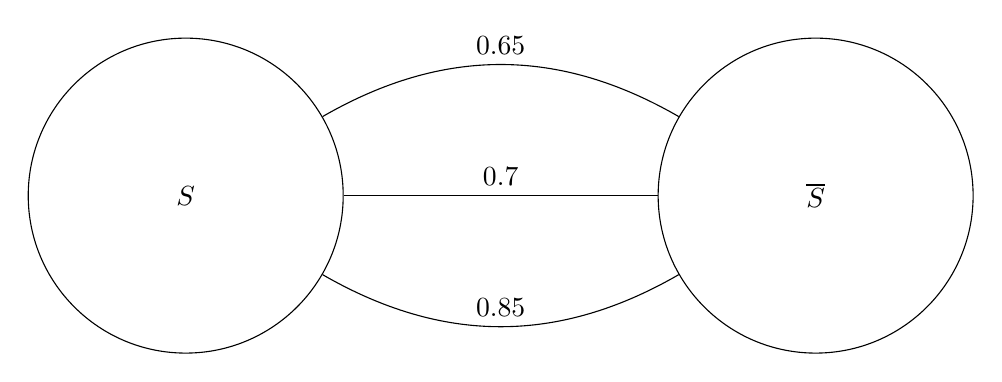
\begin{tikzpicture}
    
    \node[circle, draw=black, minimum size = 4cm] (s) at (0,0) {\(S\)};
    \node[circle, draw=black, minimum size = 4cm] (sbar) at (8,0) {\(\overline{S}\)};
    
    \path (s) edge node [above] {0.7}  (sbar); 
    \path [bend left] (s) edge node [above] {0.65} (sbar); 
    \path [bend right] (s) edge node [above] {0.85} (sbar);
    
    \end{tikzpicture}
    \caption{Solução fracionária para o TSP.}
    \label{fig:solucaoFrac}
\end{figure}

Se, no entanto, o somatório dos pesos das arestas fosse menor que 2, tanto \(S\) quanto \(\overline{S}\) estariam violando as restrições de \textit{subtour}, o que pode ser contornado adicionando-se a restrição \(\sum_{i \in S}\sum_{j \in \overline{S}}x_{ij} \geq 2\). Dessa forma, múltiplas restrições de \textit{subtour} podem ser adicionadas ao modelo antes mesmo de uma solução inteira ser obtida, além de aproximar o poliedro cada vez mais de sua envoltória convexa.

Conhecer o \textit{min-cut} do grafo que representa as soluções fracionárias da relaxação linear do TSP torna-se, portanto, uma vantagem.

\section{Algoritmos para obter o \textit{min-cut}}
O algoritmo proposto por \cite{Stoer:1997:SMA:263867.263872} é simples, e é capaz de encontrar o corte mínimo de um grafo de maneira exata. A heurística \textit{max-back} descrita em \cite{denisnaddef}, por sua vez, é mais rápida que o algoritmo exato, embora não garanta a obtenção do \textit{min-cut}. Apesar disso, para soluções inteiras, é garantido que o \textit{max-back} resolve o problema da separação.

Recomenda-se, primeiramente, o uso do \textit{max-back} na tentativa de detectar violações das restrições de \textit{subtour}. Se elas não forem encontradas, utiliza-se o algoritmo exato.

